\documentclass{article}
\usepackage{solidity}
\usepackage{hyperref}
\usepackage{graphicx}
\usepackage{float}
\usepackage[utf8]{inputenc} % For UTF-8 encoding
\usepackage{array}          % For table formatting
\usepackage{booktabs}

\usepackage{tabularx} % Include the tabularx package
\usepackage{geometry} % For adjusting page margins (if needed)

\title{Using block values as a proxy for time under Proof-of-Work vs. Proof-of-Stake Ethereum}
\author{Lorenz Kofler and Jonas Fischer}
\date{\today}
\bibliographystyle{IEEEtran}
\begin{document}
\maketitle
\tableofcontents
\newpage

%\section{Introduction}
% This paper focuses on a weakness found in Solidity smart contracts, known as 
% "block values as a proxy for time". The weakness comes from the attempt of
% developers to introduce time depended functionality in their smart contracts,
% by using the block values \textit{timestamp} and \textit{number}.

%Smart contracts often use time values to trigger some kind of action
%\cite{swc116}. Values which can be used for that are the block timestamp and
%the block number. Under PoW Ethereum using these values lead to multiple
%security issues \cite{swc116} \cite{Conkas2021} \cite{DASP2018}
%\cite{Osiris2018} \cite{Oyente2016}. Since PoS Ethereum the rules changes, this
%paper will present these changes.


\section{Introduction}

Smart contracts often utilize time values to trigger specific actions. Values
which can be employed for this purpose include the block timestamp and
the block number. However, under the Proof-of-Work consensus mechanism in
Ethereum, using these values has been associated with various security issues
\cite{swc116} \cite{Conkas2021} \cite{DASP2018} \cite{Osiris2018}
\cite{Oyente2016}.

Since the transition to the Proof-of-Stake consensus mechanism in
Ethereum, significant changes have occurred in how the timestamp value has to
be set and in the stability of the block time. This paper aims to discuss these
changes. 

The first chapter will provide an overview of Ethereum's consensus mechanism,
followed by a direct comparison of block times between Proof of Stake and
Proof of Work consensus mechanisms. Then the ppaer discuesses changes of the
usage of block.timestamp and block.number values.


\section{Overview Consensus Mechanisms}

Ethereum initially adopted the Proof-of-Work (PoW) consensus mechanism, a process known
for its security and decentralization but also criticized for its high energy
consumption and potential for centralization due to mining pools. PoW requires
miners to solve complex computational problems to validate transactions and
create new blocks, a process that consumes substantial computational power and
energy \cite{eth_pow}.

In response to these concerns, Ethereum transitioned to the Proof-of-Stake
(PoS) mechanism with "The Merge" on September 15, 2022. PoS, in contrast to
PoW, selects validators to create new blocks based on the number of coins they
hold and are willing to 'stake' as collateral. This approach significantly
reduces the energy requirements and aims to offer a more scalable and
environmentally friendly alternative \cite{eth_merge}.


\section{Block Time}

\subsection{Proof-of-Work}
\label{diff_adjustment}

In Ethereum's PoW system, the block time — the average time
interval between blocks — is primarily governed by a difficulty adjustment
algorithm. This algorithm dynamically alters the computational difficulty of
mining a block, striving to keep the block time within a targeted range.
The algorithm was implemented in the Ethereum Improvement Proposal 2 (EIP-2),
it adjusts difficulty levels based on observed block times \cite{eip-2}:

\begin{itemize}
  \item If the block time falls short of the ideal duration (less
    than 10 seconds), the difficulty is increased. This escalation in
    difficulty slows down the rate at which new blocks are mined,
    counteracting the tendency towards overly rapid block generation.

  \item Conversely, if the block time stretches beyond the desired limit (exceeding
    20 seconds), the difficulty is decreased. This reduction makes it easier to
    mine new blocks, compensating for excessively lengthy block intervals.
\end{itemize}


The follwing pie chart offers a visual representation of Ethereum's block time
distribution under PoW throughout 2021. As anticipated, the block times
exhibited considerable variability, averaging around 13.4 seconds


\begin{figure}[H]
  \centering
  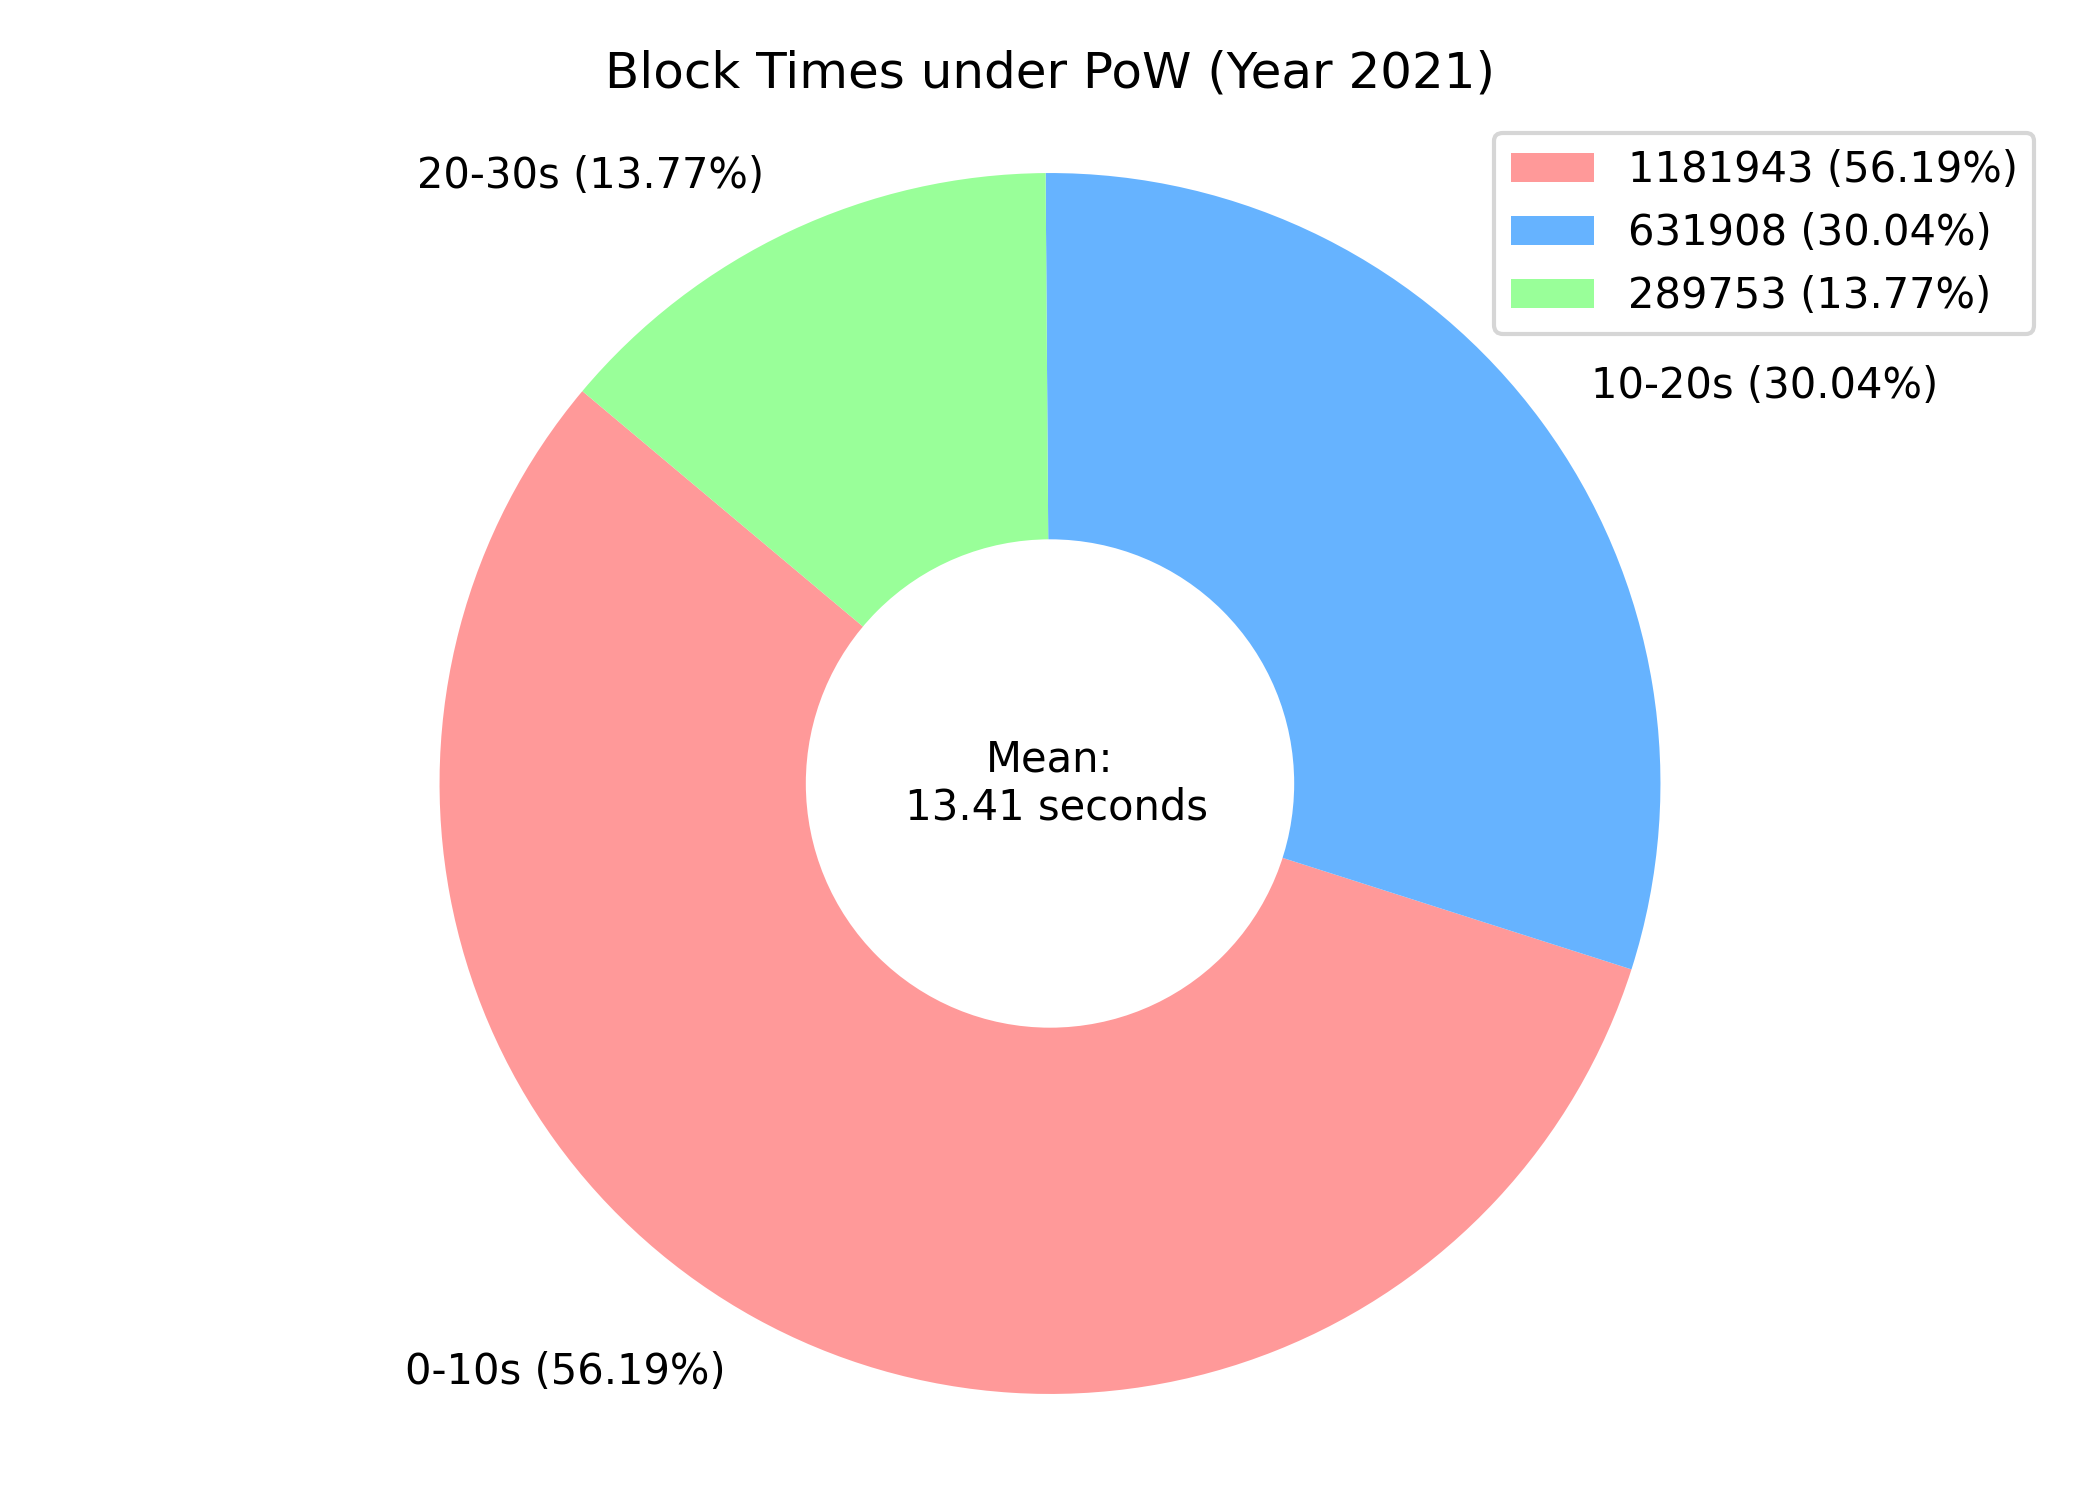
\includegraphics[width=0.8\textwidth]{block_time_analysis/pow_block_time_pie_chart.png}
  \caption{Block times under PoW in the year 2021.}
  \label{fig:block_time_analysis_pow}
\end{figure}

\subsection{Proof-of-Stake}
\label{pos_block_time}
%Following 'The Merge' on September 15, 2022, Ethereum has shifted to a
%PoS consensus mechanism \cite{eth_history}. Under PoS, validators propose new
%blocks, with a selection process involving other validators who vote to confirm
%these blocks authenticity. A stake of 32 ETH is required to be locked in as a
%deposit for one to become a validator. This staking mechanism ensures validator
%honesty, as any malpractice could lead to the loss of their staked ETH.

The newly adopted PoS system is organized around slots and epochs, with slots
being 12-second
intervals and an epoch consisting of 32 such slots
\cite{seconds-per-slot-mainnet}\cite{seconds-per-slot-mainnet-doc}. For each
slot a validator is chosen by the protocol's algorithm to propose a new block.
In the event that the selected validator, responsible for proposing a new
block, is offline, the slot remains empty
\cite{validator-offline}.

Each block within a slot corresponds to the slot's specific timestamp.
Consequently, the typical interval between blocks is approximately 12 seconds.
However, there are exceptions: if a slot remains unoccupied, the time interval
for the subsequent block extends to 24 seconds, and this pattern continues
accordingly (36,48,..).

An examination of the blockchain data since the Merge \footnote{starting at block number
15537393} reveals that 99.05\% of all blocks have been consistent with a block
time of 12 seconds, as shown in Figure
\ref{fig:block_time_analysis}.

\begin{figure}[H]
  \centering
  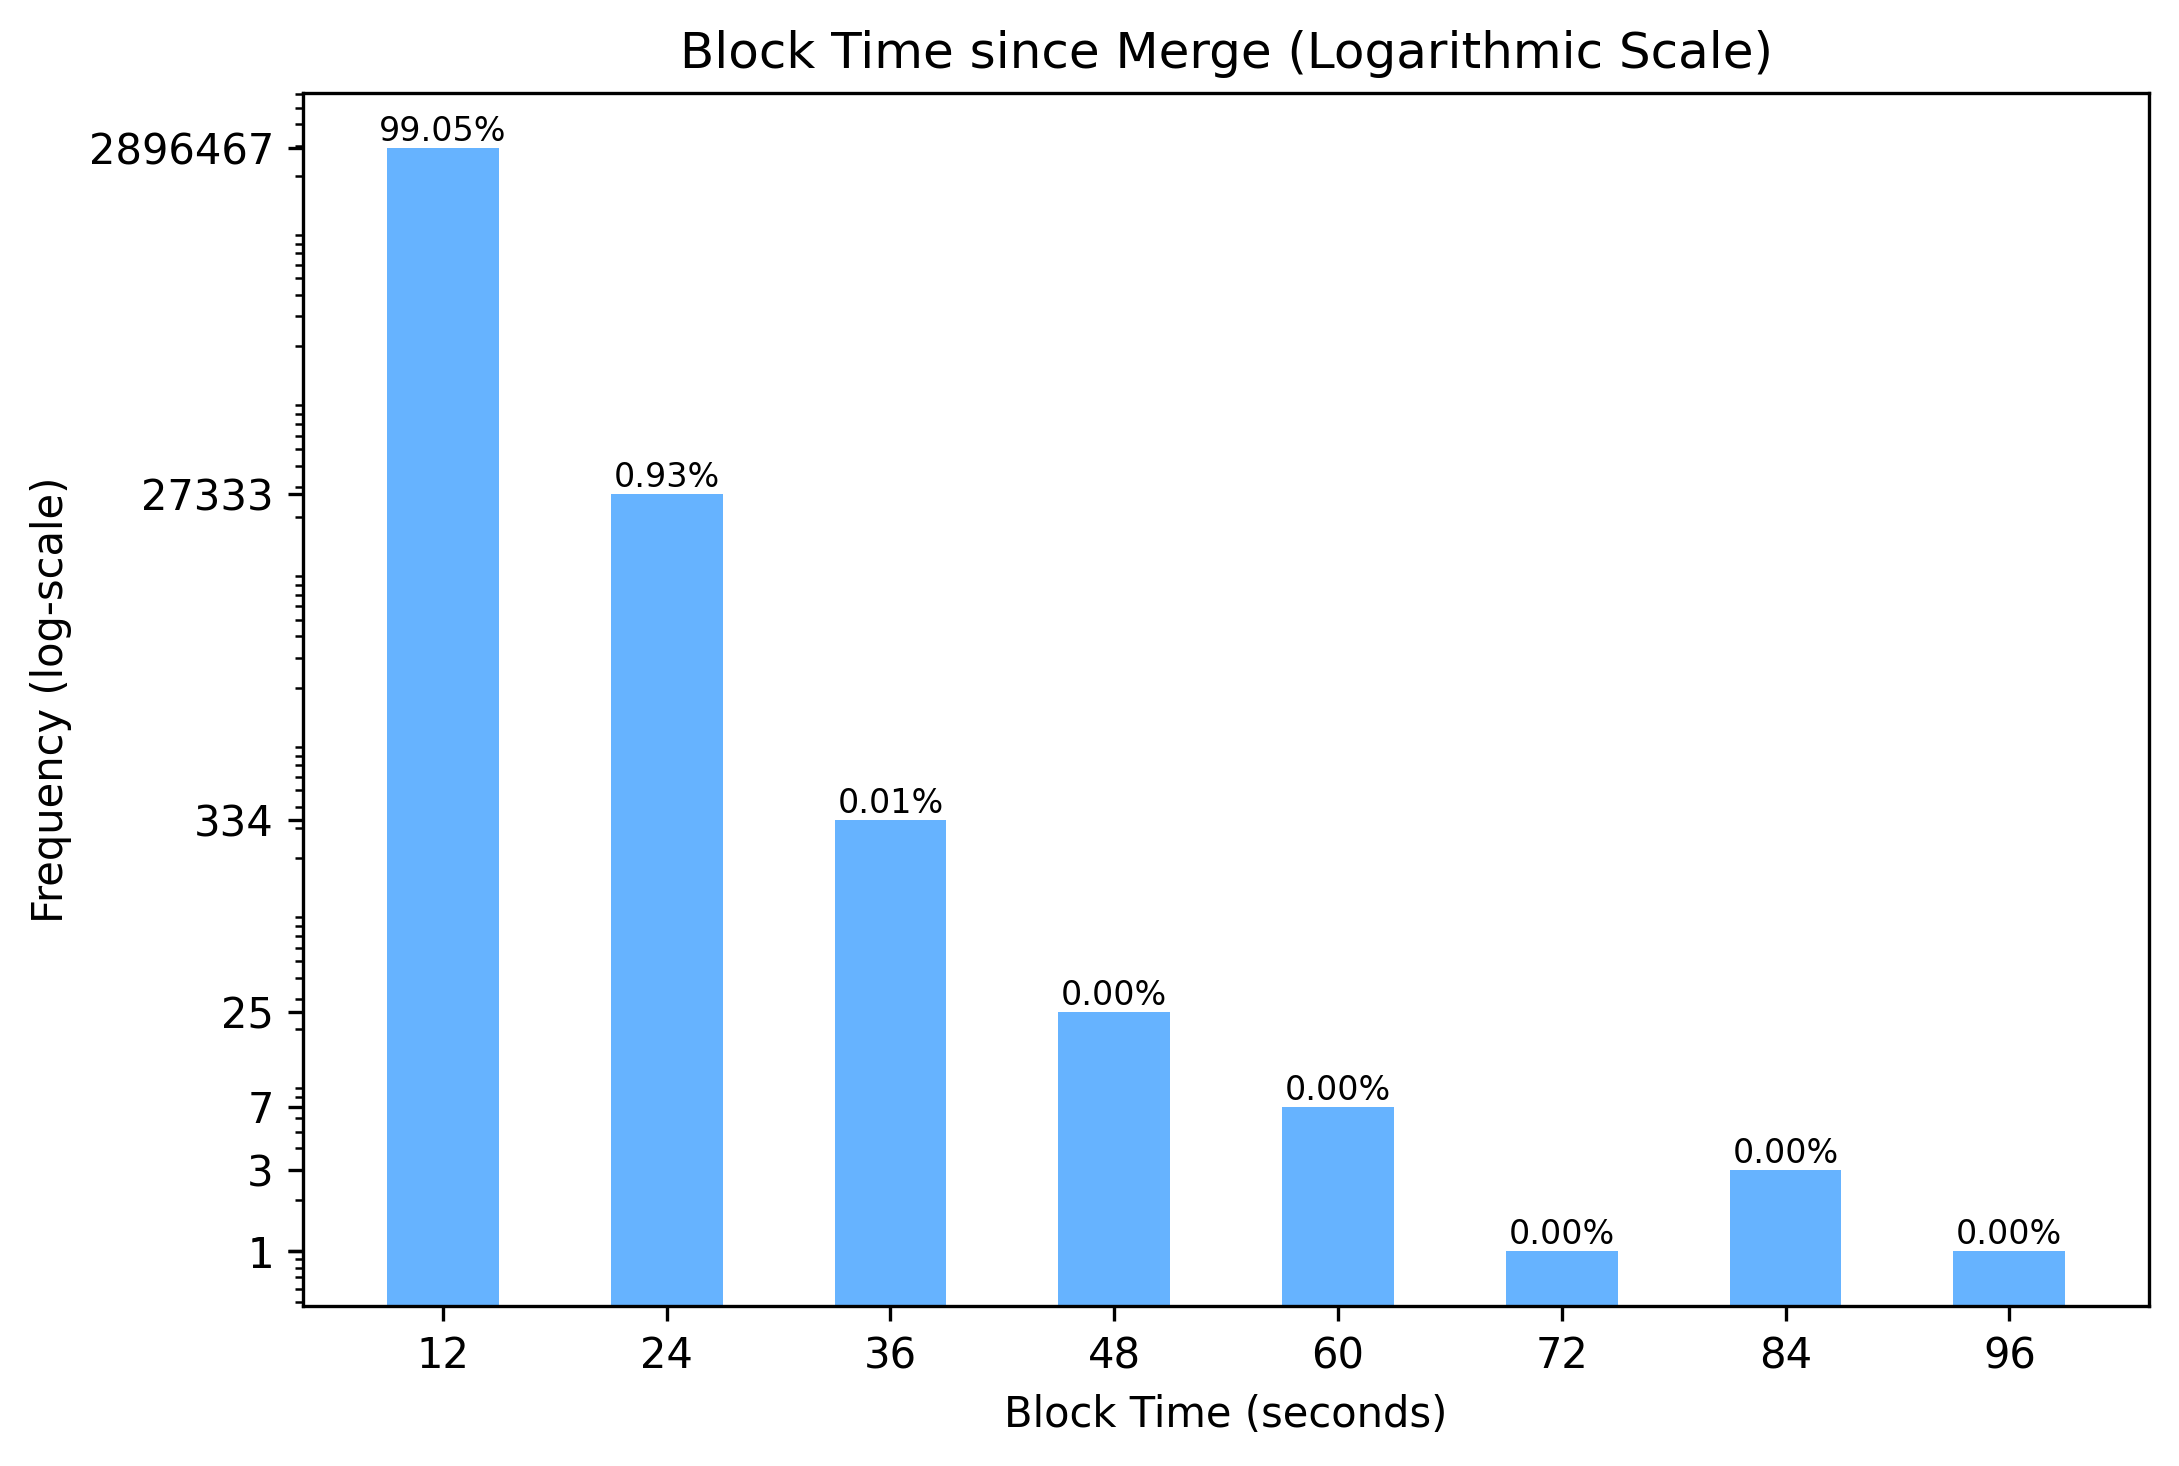
\includegraphics[width=1\textwidth]{block_time_analysis/pos_block_time_bar_chart_with_percentages.png}
  \caption{Block times since the merge.}
  \label{fig:block_time_analysis}
\end{figure}


\section{Block timestamp}

\subsection{Background} 
The miner is responsible for setting the timestamp within a block. The yellow
paper defines which rules this value has to follow. But depending on the
specific consensus mechanism there are also consensous specification and
software imposed restrictions for the timestamp value. 

\paragraph{Yellow Paper}
Pre-merge the only restriction was the yellow paper, which set that the that
the timestamp of the new block has to be greater than the timestamp of the
parent block \cite{ethyellowpaper2023}.

\paragraph{Software Implementation - Proof-of-work}
The currently most used ethereum implementation Geth rejects blocks which
timestamps are more than 15 seconds in the future
\cite{go-ethereum-15-sek-limit}. Hence when the proof-of-work consensus
mechanism was used it was possible for the miner to tamper
with the timestamp and change it up to plus 15 seconds.

\paragraph{Software Implementation - Proof-of-stake}
Proof-of-stake ethereum introduced slots, where each slot has a time frame of
12 seconds \cite{seconds-per-slot-mainnet}\cite{seconds-per-slot-mainnet-doc}.
For each slot one random validator is selected to propose a block, which other
random validatores have vote about its validity. The specification defines
how to calculate the timestamp at a specific slot with the function
\textit{compute\_timestmap\_at\_slot} \cite{compute-timestamp-at-slot}. The
timestamp is calculated with $genesis\_time + slots\_since\_genesis *
SECONDS\_PER\_SLOT$. The function \textit{process\_execution\_payload} then
checks if the blocks timestamp equals the calculated timestamp at that slot
\cite{process-execution-payload}. Hence each slot has a predefined timestamp
and it is therefore impossible to tamper with but also much more easier to
predict.
% \begin{lstlisting}[language=python, caption=proof-of-stake consensous
% specification\cite{compute-timestamp-at-slot}]
% def compute_timestamp_at_slot(state: beaconstate, slot: slot) -> uint64:
%     slots_since_genesis = slot - genesis_slot
%     return uint64(state.genesis_time + slots_since_genesis * seconds_per_slot)
% \end{lstlisting}



% \paragraph{Yellow Paper}
% Miners set the block timestamp during the mining process (source), in
% that process miners have to follow only the restriction of the Ethereum
% Yellow-Paper, which is the following:
% 
% We define $H_s$ is the timestamp of Block $H$, $P(H)$ is the parent
% block of block $H$. The Yellow-Paper defines the following relation for a valid
% block timestamp \cite{ethyellowpaper2023}.
% 
% This definition essentially means the timestamp of the block $H_s$ in
% \ref{eq:1} must be greater then the timestamp of the previous (parent) block
% $P(H)_{H_s}$ \cite{ethyellowpaper2023}.

%\paragraph{Software Implementation}
%
%\begin{lstlisting}[language=go, caption=The restriction for the timestamp in Geth. Source: \textit{consensus/ethash/consensus.go} \cite{timestamp_code}]
%func (ethash *Ethash) verifyHeader(chain consensus.ChainHeaderReader, header, parent *types.Header, uncle bool, unixNow int64) error {
%  ...
%    // Verify the header's timestamp
%        if header.Time > uint64(unixNow+allowedFutureBlockTimeSeconds) {
%            return consensus.ErrFutureBlock
%        }
%    if header.Time <= parent.Time {
%        return errOlderBlockTime
%    }
%  ...
%}
%\end{lstlisting}
%
%\paragraph{Issues}

\begin{itemize}
\item Do not use block.timestamp as time locks, since developer should follow the yellow paper, it is not sure that software implements the restrictions.
\item Do not use block.timestamp as a source of randomness.
\end{itemize}

\subsection{Examples}
\subsubsection{Example containing weakness}
\begin{solidity}
contract Firework {
    function startFirework() public {
        // 01.01.2024 00:00:00 GMT+0100
        require(block.timestamp > 1704063600);
    }
}
\end{solidity}

\subsubsection{Example without a weakness}
\begin{solidity}
contract Game {
    uint expiry;

    constructor(uint expiryTimestamp) public {
        expiry = expiryTimestamp;
    }

    function play() public {
        // Safe to use because block timestamp can not be modified backwards
        require(block.timestamp < expiry);
    }
}
\end{solidity}
    
\subsection{Consequences}
A miner is gaining an unfair advantage if he is able to set the timestamp
of his mined block into the future, such that he is able to access
resources earlier then other users or trigger events before they are meant to happen.

\section{Block number}
\subsection{Proof-of-Work}
The yellow paper of Ethereum states that each block has
an integer value as a block number. The block number
of a specific block must be exactly one unit higher than the block
number of the previous block \cite{ethyellowpaper2023}.
Smart contract developers attempted to utilize the block number to calculate
the current time, operating under the assumption that the time interval between
two blocks always remains constant at fourteen seconds. Theoretically, one could
calculate time differences between blocks by multiplying the block numbers by fourteen 
and subtracting them from each other.
However, this approach proves impractical in reality due to the variable
intervals between blocks, as explained earlier. Moreover, these block intervals
can change unexpectedly, for instance, when the difficulty bomb was introduced
or during a chain fork \cite{swc116}.
As a result the block number should not be used as a proxy for time.
%An example for this misusage can be seen in the Listing \ref{lst:number_weakness}.
%There the block number is used to lock a function of a contract for a specific time.

%\lstinputlisting[language=Solidity, caption={Block Number Weakness in PoW},linerange={4-17}, label={lst:number_weakness}]{../dev/contracts/blocknumbertimelock.sol}

\subsection{Proof-of-Stake}
In PoS, just like in PoW, the block number increases by one with each new
block. In PoS, the block intervals are for 99.05\% of times at 12 seconds. Consequently,
it might appear that using the block number as a time proxy in PoS is a viable
option. However, it's not advisable, because validators go offline from time to
time. This causes the block time to increase and therefore leads to an
inaccuracy of the calculation of time based on the block number. \\
% (like the one in Listing \ref{lst:number_weakness})
A contract initially deployed under PoW would
become impractical or malfunction in a PoS environment due to the inherent differences in the block times.

\subsection{Summary}
The transition from PoW to PoS has significantly stabilized block times,
particularly over short periods. However, it's important to note that using
the block number as a proxy for time is still not advisable, as the fixed value
with 
12 seconds per slot might change in the future. In earlier PoS designs, the
slot time was set at 6 seconds \cite{block_time_6_to_12_sec}. There have
also been proposals to adjust the slot time to 8 seconds
\cite{proposed_block_time_8_seconds}. This indicates that for shorter
durations, block times under PoS are markedly more stable than those under
PoW. Conversely, for longer timeframes, this stability is less assured due
to the potential for changes in slot time.



\section{Conclusion}

Under PoW miners were able to manipulate block timestamps for a up 15 seconds.
Consequently, utilizing the block timestamp for time-dependent events was
secure only if the contract's time-dependent events could tolerate a variation
of up to 15 seconds while still maintaining their integrity. Since PoS
timestamp manipulation is impossible and therefore secure to use since miners
can not gain an unfair advantage by modifing the timestamp.

In PoW Ethereum, block times were probabilistic since they are influenced by
the mining difficulty. In contrast, block times under PoS are significantly more
consistent, mostly 12 seconds, compared to those in PoW. Therefore, in PoS,
using block numbers as a measure of time is generally more accurate than in
PoW, especially for shorter durations (possibly less than a year). However,
it's important to note that the fixed block time (slot time) in PoS is not
guaranteed to remain unchanged indefinitely. Therefore, using block numbers as
a time proxy is generally not advisable.


%In PoW-based Ethereum, block times were probabilistic and influenced by mining difficulty.
%As a result, using block values as a time proxy in PoW was not secure.
%However, since Ethereum's transition to PoS, this is no longer the case.
%PoS-based Ethereum has fixed block times of 12 seconds or multiples thereof.
%Our research has shown that block times can no longer be influenced from external sources.
%Therefore, using the block.timestamp value as a time proxy is now safe in PoS.
%
%Using the block.number as a proxy for time is still not advisable. Block times 
%can become a multiple of 12s and it is also not guaranteed that the block intervals will
%never change again in the future.


\section{Use-cases}

\subsection{Timelocks}
A timelock is a smart contract that serves as a mechanism to delay function calls form another contract for
a predefined amount of time. Timelocks find their primary application in governance systems,
where they play a crucial role in implementing delayed administrative actions.
Their presence often signifies the credibility of a project and underscores the commitment of its owners
to its long-term success. \cite{timelock2021}.

Openzeppelin provides such a timelock in their library (@openzeppelin/contracts/governance/TimelockController.sol).
A part of this timelock code can be seen in Listing \ref{lst:timelock} \cite{timelock_code}.

\lstinputlisting[language=Solidity, caption={Openzeppelin Timelock}, label={lst:timelock}]{../dev/contracts/timelock.sol}

\subsection{State Machine}
Contracts often act as a state machine. It's common to have multi-stage
processes where certain actions are allowed only during specific phases.
Timestamps can be used to enforce time-based conditions within a contract \cite{soliditydocs_statemaschine}. \\
The following example shows a contract that implements the transition of stages (states) based on timestamps \cite{stagedcontract_code}.

\begin{solidity}
modifier timedTransitions() {
    if (stage == Stages.AcceptingBlindBids && block.timestamp >= creationTime + 6 days) {
        nextStage();
    }
    if (stage == Stages.RevealBids && block.timestamp >= creationTime + 10 days) {
        nextStage();
    }
    _;
}
\end{solidity}

\section{Best practices}
- Avoid using block.number in PoW as a proxy for time, because it is not guaranteed that the block time is fixed at 14 seconds \\
- Avoid using block.number in PoS as a proxy for time, because the block time can be a multiple of 12 seconds and may change in the future (instead use block.timestamp)\\
- Avoid using block.timestamp in PoW, because it can be manipulated by miners \\
- Avoid using block.timestamp in PoS for triggering events with an exact time (more accurate than 12 seconds, e.g. silvester) \\
- It is safe to use block.timestamp in PoS, if the time-dependent event must only be higher than a certain timestamp (e.g. timelocks) \\

%\section{Introduction}

Smart contracts often utilize time values to trigger specific actions. The
values that can be employed for this purpose include the block timestamp and
the block number. However, under the Proof of Work (PoW) consensus mechanism in
Ethereum, using these values has been associated with various security issues
\cite{swc116} \cite{Conkas2021} \cite{DASP2018} \cite{Osiris2018}
\cite{Oyente2016}.


Since the transition to the Proof of Stake (PoS) consensus mechanism in
Ethereum, significant changes have occurred in how the timestamp value has to
be set and in the stability of the block time. This paper aims to discuss these
changes.

\section{Ethereum's Consensus Mechanisms}
Ethereum initially adopted the Proof of Work (PoW) mechanism, a process known
for its security and decentralization but also criticized for its high energy
consumption and potential for centralization due to mining pools. PoW requires
miners to solve complex computational problems to validate transactions and
create new blocks, a process that consumes substantial computational power and
energy.

In response to these concerns, Ethereum transitioned to the Proof of Stake
(PoS) mechanism with "The Merge" on September 15, 2022. PoS, in contrast to
PoW, selects validators to create new blocks based on the number of coins they
hold and are willing to 'stake' as collateral. This approach significantly
reduces the energy requirements and aims to offer a more scalable and
environmentally friendly alternative.


\section{Block Time in Ethereum}

\subsection{Proof-of-Work block time}

In Ethereum's Proof-of-Work (PoW) system, the block time — the average time
interval between blocks — is primarily governed by a difficulty adjustment
algorithm. This algorithm dynamically alters the computational difficulty of
mining a block, striving to keep the block time within a targeted range.
According to Ethereum Improvement Proposal 2 (EIP-2), the algorithm adjusts
difficulty levels based on observed block times \cite{eip-2}:

\begin{itemize}
  \item If the block time falls short of the ideal duration (less
    than 10 seconds), the difficulty is increased. This escalation in
    difficulty slows down the rate at which new blocks are mined,
    counteracting the tendency towards overly rapid block generation.

  \item Conversely, if the block time stretches beyond the desired limit (exceeding
    20 seconds), the difficulty is decreased. This reduction makes it easier to
    mine new blocks, compensating for excessively lengthy block intervals.
\end{itemize}


The following pie chart provides a graphical depiction of Ethereum's block time
distribution under the Proof of Work (PoW) mechanism for the year 2021,
highlighting significant fluctuations, with an average block time of
approximately 13.4 seconds.


\begin{figure}[H]
  \centering
  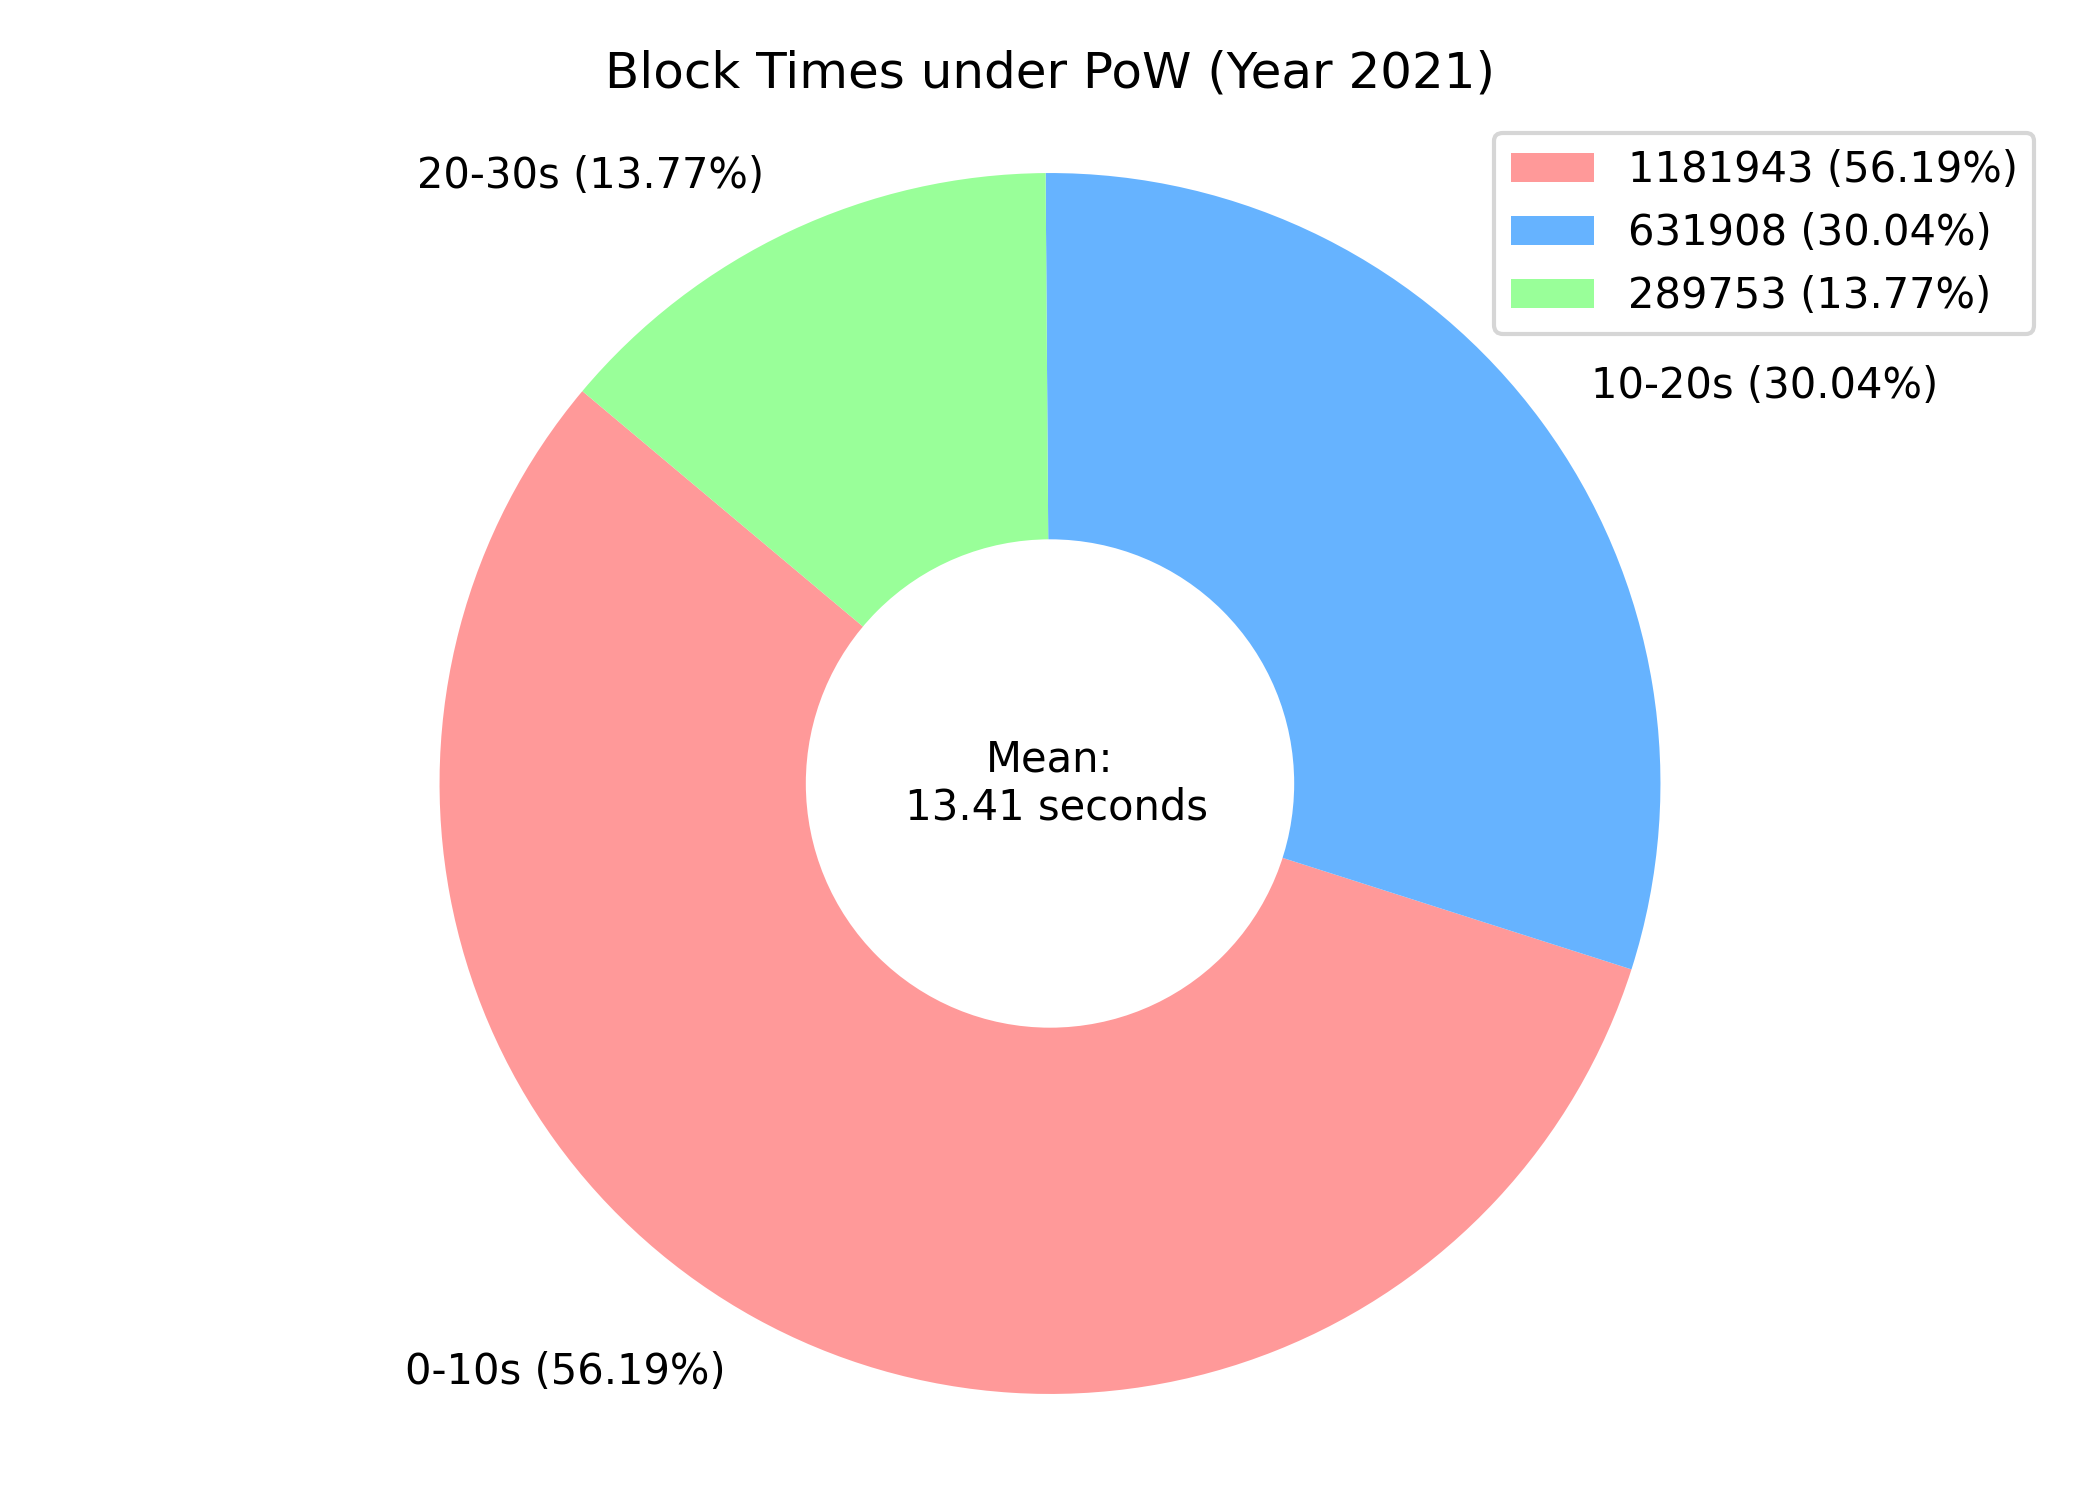
\includegraphics[width=0.8\textwidth]{block_time_analysis/pow_block_time_pie_chart.png}
  \caption{Block times under PoW in the year 2021.}
  \label{fig:block_time_analysis_pow}
\end{figure}

\subsection{Proof-of-Stake block time}
Since "The Merge" on September 15, 2022, Ethereum has transitioned to a
Proof-of-Stake (PoS) consensus protocol. In PoS Ethereum, new blocks are
proposed by validators, and then randomly selected validators must vote on the
validity of these proposed blocks. To become a validator, a deposit of 32 ETH
is required, stored in a deposit contract. Validators are incentivized to act
honestly as they risk losing a portion or all of their staked ETH if they
behave dishonestly.

Proof-of-stake Ethereum introduced the concepts of slots and epochs. Each slot
has a time frame of 12 seconds, and an epoch spans 32 slots
\cite{seconds-per-slot-mainnet}\cite{seconds-per-slot-mainnet-doc}. In each
slot, one validator is randomly chosen to propose a new block to the network.
Validators are required to adhere to the protocol's specifications when
creating new blocks; otherwise, their blocks will be rejected.

\begin{figure}[H]
  \centering
  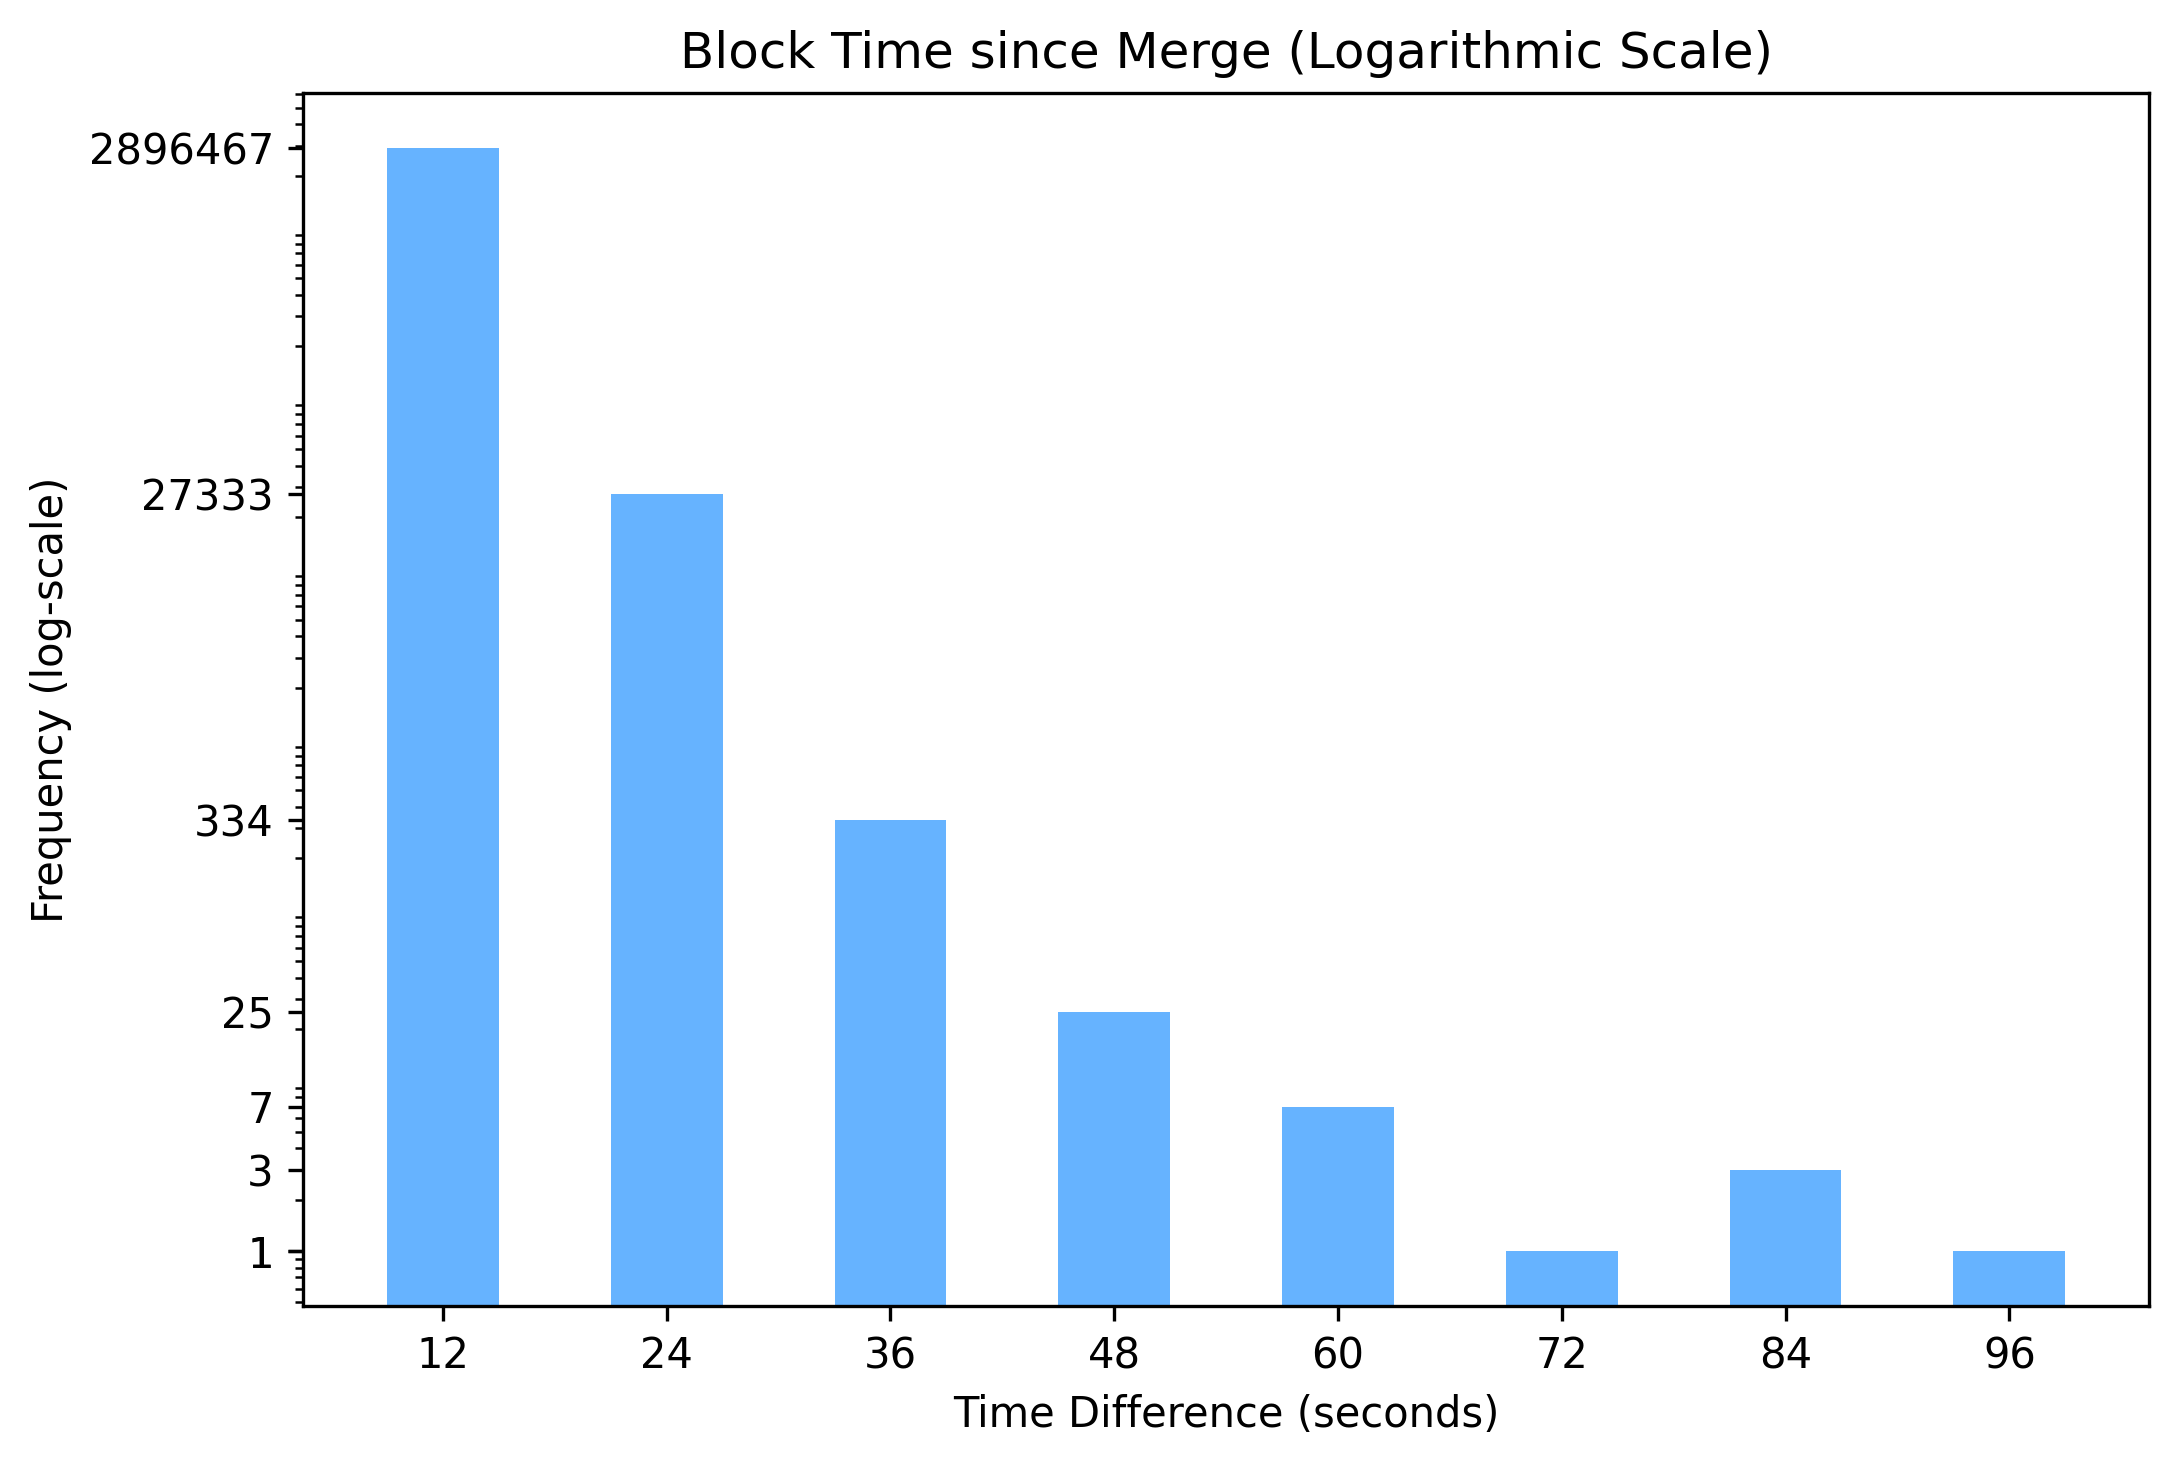
\includegraphics[width=1\textwidth]{block_time_analysis/pos_block_time_bar_chart.png}
  \caption{Block times since the merge.}
  \label{fig:block_time_analysis}
\end{figure}

\section{Block timestamp in Ethereum}
\subsection{Proof-of-Work Block Timestamp}
As a result of the difficulty adjustment algorithm, the block time had the
potential to vary from one block to another. Furthermore, the only restriction
miners had to follow when setting the block timestamp value was outlined in the
yellow paper, which stipulated that the timestamp of the new block must be
greater than the timestamp of the parent block \cite{ethyellowpaper2023}.
Consequently, miners could gain an unfair advantage by manipulating the
timestamp of their mined block (references to be added).


To prevent miners from setting the timestamp too far into the future, some of the most widely used Ethereum implementations, such as Geth (go-ethereum), implemented a rejection mechanism for blocks with timestamps exceeding 15 seconds into the future \cite{go-ethereum-15-sek-limit}.

Hence, when the PoW consensus mechanism was in use, miners had the ability to
manipulate the timestamp and adjust it by up to 15 seconds. This behavior led
to the establishment of the "15-second Rule"
\footnote{\url{https://consensys.github.io/smart-contract-best-practices/development-recommendations/solidity-specific/timestamp-dependence/}},
as a security best practice. The
rule suggests that the usage of the block timestamp is considered
safe if the time-dependent event can tolerate a variation of up to 15 seconds. 

\subsection{Proof-of-Stake Block Timestamp}

The PoS Ethereum consensus specification provides instructions on how to
calculate the timestamp at a specific slot using the
\textit{compute\_timestamp\_at\_slot} function \cite{compute-timestamp-at-slot}.
This calculation is based on the following formula:

\begin{equation}
genesis\_time + slots\_since\_genesis *
seconds\_per\_slot
\end{equation}


In the Ethereum mainnet configuration, the value of \textit{seconds\_per\_slot} is set to
12 seconds \cite{seconds-per-slot-mainnet} \cite{seconds-per-slot-mainnet-doc}.
The mainnet beacon chain's value for \textit{genesis\_time} is $1606824023$, which
corresponds to the timestamp when the original PoS beacon chain was launched on
December 1, 2020.

Each validator calculates the block timestamp in the same way and verifies if
the timestamp in the block matches the calculated timestamp. If there is a
mismatch, the block is rejected \cite{process-execution-payload}. Since each
slot, and consequently each block, has a predetermined timestamp, it is
virtually impossible to tamper with, but it also becomes more predictable. In
the event that the selected validator, responsible for proposing a new block,
is offline, the slot remains empty \cite{validator-offline}. The timestamp of
the following block aligns with the timestamp of the following slot, which is a
multiple of \textit{SECONDS\_PER\_SLOT}. As a result, blocks are 24 seconds
apart. If subsequent validators are also offline, the block times will be 36
seconds apart, and so on.

Analyzing blockchain data (refer to Figure \ref{fig:block_time_analysis}) following the
merge (block number $> 15537393$) shows that 99.05 \% of all blocks exhibit a
block time of 12 seconds.

\section{Block number in Ethereum}
\subsection{Proof-of-Work Block Number}
The yellow paper of Ethereum states that each block has
an integer value as a block number. The block number
of a specific block must be exactly one unit higher than the block
number of the previous block \cite{ethyellowpaper2023}.
Smart contract developers attempted to utilize the block number to calculate
the current time, operating under the assumption that the time interval between
two blocks always remains constant at fourteen seconds. Theoretically, one could
calculate time differences between blocks by multiplying the block numbers by fourteen 
and subtracting them from each other.
However, this approach proves impractical in reality due to the variable
intervals between blocks, as explained earlier. Moreover, these block intervals
can change unexpectedly, for instance, when the difficulty bomb was introduced
or during a chain fork \cite{swc116}.
As a result the block number should not be used as a proxy for time.
An example for this misusage can be seen in the Listing \ref{lst:number_weakness}.
There the block number is used to lock a function of a contract for a specific time.

\lstinputlisting[language=Solidity, caption={Block Number Weakness in PoW},linerange={4-17}, label={lst:number_weakness}]{../dev/contracts/bad-blocknumber.sol}

\subsection{Proof-of-Stake Block Number}
In PoS, just like in PoW, the block number increases by one with each new block.
In PoS, the block intervals are consistently set at 12 seconds.
Consequently, it might appear that using the block number as a time proxy in PoS is a viable option. 
However, it's not advisable, because validators go offline from time to time.
This causes the block time to increase and therefore leads to an inaccuracy of the calculation
of time based on the block number.


\section{Conclusion: Block Time under PoW vs. PoS}
In PoW-based Ethereum, block times were probabilistic and influenced by mining difficulty.
As a result, using block values as a time proxy in PoW was not secure.
However, since Ethereum's transition to PoS, this is no longer the case.
PoS-based Ethereum has fixed block times of 12 seconds or multiples thereof.
Our research has shown that block times can no longer be influenced from external sources.
Therefore, using the block.timestamp value as a time proxy is now safe in PoS.

Using the block.number as a proxy for time is still not advisable. Block times 
can become a multiple of 12s and it is also not guaranteed that the block intervals will
never change again in the future.

%\section{Block number}
\subsection{Proof-of-Work}
The yellow paper of Ethereum states that each block has
an integer value as a block number. The block number
of a specific block must be exactly one unit higher than the block
number of the previous block \cite{ethyellowpaper2023}.
Smart contract developers attempted to utilize the block number to calculate
the current time, operating under the assumption that the time interval between
two blocks always remains constant at fourteen seconds. Theoretically, one could
calculate time differences between blocks by multiplying the block numbers by fourteen 
and subtracting them from each other.
However, this approach proves impractical in reality due to the variable
intervals between blocks, as explained earlier. Moreover, these block intervals
can change unexpectedly, for instance, when the difficulty bomb was introduced
or during a chain fork \cite{swc116}.
As a result the block number should not be used as a proxy for time.
%An example for this misusage can be seen in the Listing \ref{lst:number_weakness}.
%There the block number is used to lock a function of a contract for a specific time.

%\lstinputlisting[language=Solidity, caption={Block Number Weakness in PoW},linerange={4-17}, label={lst:number_weakness}]{../dev/contracts/blocknumbertimelock.sol}

\subsection{Proof-of-Stake}
In PoS, just like in PoW, the block number increases by one with each new
block. In PoS, the block intervals are for 99.05\% of times at 12 seconds. Consequently,
it might appear that using the block number as a time proxy in PoS is a viable
option. However, it's not advisable, because validators go offline from time to
time. This causes the block time to increase and therefore leads to an
inaccuracy of the calculation of time based on the block number. \\
% (like the one in Listing \ref{lst:number_weakness})
A contract initially deployed under PoW would
become impractical or malfunction in a PoS environment due to the inherent differences in the block times.

\subsection{Summary}
The transition from PoW to PoS has significantly stabilized block times,
particularly over short periods. However, it's important to note that using
the block number as a proxy for time is still not advisable, as the fixed value
with 
12 seconds per slot might change in the future. In earlier PoS designs, the
slot time was set at 6 seconds \cite{block_time_6_to_12_sec}. There have
also been proposals to adjust the slot time to 8 seconds
\cite{proposed_block_time_8_seconds}. This indicates that for shorter
durations, block times under PoS are markedly more stable than those under
PoW. Conversely, for longer timeframes, this stability is less assured due
to the potential for changes in slot time.



% \begin{tikzpicture}
    \begin{axis}[
      height=10cm,
      ymin = 0,
      xtick=data,
      xticklabels from table={\datatable}{Date(UTC)},
      x tick label style={font=\normalsize, rotate=90, anchor=east},
      ylabel={Average Block Time (s)}]
      \addplot table [x expr=\coordindex, y={AverageBlockTime}]{\datatable};
    \end{axis}
\end{tikzpicture}

%\section{Vulnerable contracts}

\begin{solidity}[caption=NCC Group - Time manipulation \cite{DASP2018}]
    function play() public {
        require(block.timestamp > 1521763200 && neverPlayed == true);
        neverPlayed = false;
        msg.sender.transfer(1500 ether);
    }
\end{solidity}

\begin{solidity}[caption=SWC116 \cite{swc116}]
contract TimeLock {
    struct User {
        uint amount; // amount locked (in eth)
        uint unlockBlock; // minimum block to unlock eth
    }

    mapping(address => User) private users;

    // Tokens should be locked for exact time specified
    function lockEth(uint _time, uint _amount) public payable {
        require(msg.value == _amount, 'must send exact amount');
        users[msg.sender].unlockBlock = block.number + (_time / 14);
        users[msg.sender].amount = _amount;
    }

    // Withdraw tokens if lock period is over
    function withdraw() public {
        console.log("Trying to withdraw");

        require(users[msg.sender].amount > 0, 'no amount locked');
        require(block.number >= users[msg.sender].unlockBlock, 'lock period not over');

        uint amount = users[msg.sender].amount;
        users[msg.sender].amount = 0;
        (bool success, ) = msg.sender.call.value(amount)("");

        console.log("Withdraw done");

        require(success, 'transfer failed');
    }
}
\end{solidity}

% \begin{solidity}[caption=Timestamp depended contract \cite{SmartCheck2018}]
%     if (block.timestamp \% 2 == 0) winner = pl1 ; else winner = pl2;
% \end{solidity}

% \begin{solidity}[caption=The Run smart contract \cite{therun_contract}]
%     uint256 constant private salt =  block.timestamp;
%     
%     function random(uint Max) constant private returns (uint256 result){
%         //get the best seed for randomness
%         uint256 x = salt * 100 / Max;
%         uint256 y = salt * block.number / (salt % 5) ;
%         uint256 seed = block.number/3 + (salt % 300) + Last_Payout +y; 
%         uint256 h = uint256(block.blockhash(seed)); 
%     
%         return uint256((h / x)) % Max + 1; //random number between 1 and Max
%     }
% \end{solidity}

%\section{Tools and code properties}

\subsection{conkas}
Conkas checks if a variable in the code is called 'timestamp' \cite{conkas_opcodes} \newline
\begin{lstlisting}
    TIME_MANIPULATION_VAR = 'timestamp'
    def __is_based_on_time(data):
    for var in get_vars(data):
        var_name = str(var)
        if var_name == TIME_MANIPULATION_VAR:
            return True
        return False
\end{lstlisting}

\begin{lstlisting}[language=bash, caption="conkas output for the timed\_crowdsale.sol contract"]
    ==== Dependence on predictable environment variable ====
    SWC ID: 116
    Severity: Low
    Contract: TimedCrowdsale
    Function name: run()
    PC address: 98
    Estimated Gas Usage: 176 - 271
    A control flow decision is made based on The block.timestamp environment variable.
    The block.timestamp environment variable is used to determine a control flow decision. Note that the values of variables like coinbase, gaslimit, block number and timestamp are predictable and can be manipulated by a malicious miner. Also keep in mind that attackers know hashes of earlier blocks. Don't use any of those environment variables as sources of randomness and be aware that use of these variables introduces a certain level of trust into miners.
    --------------------
    In file: /contracts/timed_crowdsale.sol:14    
\end{lstlisting}

\subsection{mythril}
Mythril looks for the opcodes TIMESTAMP and NUMBER in the code and warns the user if they are found \cite{mythril_opcodes}. \newline
\verb|predictable_ops = ["COINBASE", "GASLIMIT", "TIMESTAMP", "NUMBER"]|

\begin{lstlisting}[language=bash, caption="Mythril output for the time lock contract"]
==== Dependence on predictable environment variable ====
SWC ID: 120
Severity: Low
Contract: TimeLock
Function name: withdraw()
PC address: 697
Estimated Gas Usage: 1985 - 2460
A control flow decision is made based on The block.number environment variable.
The block.number environment variable is used to determine a control flow decision. Note that the values of variables like coinbase, gaslimit, block number and timestamp are predictable and can be manipulated by a malicious miner. Also keep in mind that attackers know hashes of earlier blocks. Don't use any of those environment variables as sources of randomness and be aware that use of these variables introduces a certain level of trust into miners.
--------------------
In file: /contracts/time_lock.sol:25

require(block.number >= users[msg.sender].unlockBlock, 'lock period not over')
\end{lstlisting}
%\section{Exploits}
%\section{Block timestamp}

\subsection{Background} 
The miner is responsible for setting the timestamp within a block. The yellow
paper defines which rules this value has to follow. But depending on the
specific consensus mechanism there are also consensous specification and
software imposed restrictions for the timestamp value. 

\paragraph{Yellow Paper}
Pre-merge the only restriction was the yellow paper, which set that the that
the timestamp of the new block has to be greater than the timestamp of the
parent block \cite{ethyellowpaper2023}.

\paragraph{Software Implementation - Proof-of-work}
The currently most used ethereum implementation Geth rejects blocks which
timestamps are more than 15 seconds in the future
\cite{go-ethereum-15-sek-limit}. Hence when the proof-of-work consensus
mechanism was used it was possible for the miner to tamper
with the timestamp and change it up to plus 15 seconds.

\paragraph{Software Implementation - Proof-of-stake}
Proof-of-stake ethereum introduced slots, where each slot has a time frame of
12 seconds \cite{seconds-per-slot-mainnet}\cite{seconds-per-slot-mainnet-doc}.
For each slot one random validator is selected to propose a block, which other
random validatores have vote about its validity. The specification defines
how to calculate the timestamp at a specific slot with the function
\textit{compute\_timestmap\_at\_slot} \cite{compute-timestamp-at-slot}. The
timestamp is calculated with $genesis\_time + slots\_since\_genesis *
SECONDS\_PER\_SLOT$. The function \textit{process\_execution\_payload} then
checks if the blocks timestamp equals the calculated timestamp at that slot
\cite{process-execution-payload}. Hence each slot has a predefined timestamp
and it is therefore impossible to tamper with but also much more easier to
predict.
% \begin{lstlisting}[language=python, caption=proof-of-stake consensous
% specification\cite{compute-timestamp-at-slot}]
% def compute_timestamp_at_slot(state: beaconstate, slot: slot) -> uint64:
%     slots_since_genesis = slot - genesis_slot
%     return uint64(state.genesis_time + slots_since_genesis * seconds_per_slot)
% \end{lstlisting}



% \paragraph{Yellow Paper}
% Miners set the block timestamp during the mining process (source), in
% that process miners have to follow only the restriction of the Ethereum
% Yellow-Paper, which is the following:
% 
% We define $H_s$ is the timestamp of Block $H$, $P(H)$ is the parent
% block of block $H$. The Yellow-Paper defines the following relation for a valid
% block timestamp \cite{ethyellowpaper2023}.
% 
% This definition essentially means the timestamp of the block $H_s$ in
% \ref{eq:1} must be greater then the timestamp of the previous (parent) block
% $P(H)_{H_s}$ \cite{ethyellowpaper2023}.

%\paragraph{Software Implementation}
%
%\begin{lstlisting}[language=go, caption=The restriction for the timestamp in Geth. Source: \textit{consensus/ethash/consensus.go} \cite{timestamp_code}]
%func (ethash *Ethash) verifyHeader(chain consensus.ChainHeaderReader, header, parent *types.Header, uncle bool, unixNow int64) error {
%  ...
%    // Verify the header's timestamp
%        if header.Time > uint64(unixNow+allowedFutureBlockTimeSeconds) {
%            return consensus.ErrFutureBlock
%        }
%    if header.Time <= parent.Time {
%        return errOlderBlockTime
%    }
%  ...
%}
%\end{lstlisting}
%
%\paragraph{Issues}

\begin{itemize}
\item Do not use block.timestamp as time locks, since developer should follow the yellow paper, it is not sure that software implements the restrictions.
\item Do not use block.timestamp as a source of randomness.
\end{itemize}

\subsection{Examples}
\subsubsection{Example containing weakness}
\begin{solidity}
contract Firework {
    function startFirework() public {
        // 01.01.2024 00:00:00 GMT+0100
        require(block.timestamp > 1704063600);
    }
}
\end{solidity}

\subsubsection{Example without a weakness}
\begin{solidity}
contract Game {
    uint expiry;

    constructor(uint expiryTimestamp) public {
        expiry = expiryTimestamp;
    }

    function play() public {
        // Safe to use because block timestamp can not be modified backwards
        require(block.timestamp < expiry);
    }
}
\end{solidity}
    
\subsection{Consequences}
A miner is gaining an unfair advantage if he is able to set the timestamp
of his mined block into the future, such that he is able to access
resources earlier then other users or trigger events before they are meant to happen.


\newpage
\bibliography{seminar}
\end{document}
